\documentclass{report}
\usepackage{graphicx} % Required for inserting images
\usepackage{geometry}
\usepackage{amsmath}
\usepackage{mathtools}
\usepackage{amssymb}
\usepackage{kotex}
\usepackage{makecell}
\usepackage{bytefield}
\usepackage{listings}
\usepackage{caption}
\usepackage{subcaption}

\captionsetup{labelformat=empty,labelsep=none,font=small}
\lstset{
    basicstyle=\small\ttfamily,
    commentstyle=\small\ttfamily,
    numbers=left,
    columns=flexible,
    breaklines=true,
    captionpos=b,
    xleftmargin=5.0ex,
    aboveskip=1.0em,
}

\title{CSED551 PA\#2 \\[0.5ex] {\normalsize :Frequency Domain Processing}}
\author{\small{20220848 Minsu Sun}}
\date{\small{October 20, 2024}}

\begin{document}

\maketitle

\section*{Problem 1}

\subsection*{Algorithm - Primitives}

아래는 Ideal Lowpass Filtering을 구현함에 있어서 필요함에 따라 작성한 함수들에 대한 설명이다.

\begin{lstlisting}[language=Python, caption=Primitive - squaredDistanceMatrix, firstnumber=7]
def squaredDistanceMatrix(shape: tuple[int, int]) -> "np.ndarray[np.float32]":
    """Get squared distance matrix shaped of given shape

    Args:
        shape (tuple[int, int]): shape of desired distance matrix

    Returns:
        np.ndarray[np.float32]: squared distance matrix
    """
    u: np.ndarray[np.float32] = (
        np.arange(shape[0]).astype(np.float32) - (shape[0] - 1) / 2
    )
    v: np.ndarray[np.float32] = (
        np.arange(shape[1]).astype(np.float32) - (shape[1] - 1) / 2
    )
    U: np.ndarray[np.float32]
    V: np.ndarray[np.float32]
    V, U = np.meshgrid(v, u)  # U, V are both shaped like (u.shape[0], v.shape[0])
    return U**2 + V**2  # distance^2 matrix from the middle
\end{lstlisting}

위의 코드는 매개변수로 주어진 \code{shape}의 형태에 맞춘 Distance Matrix $D$의 각 원소들의 제곱으로 이루어진 $D^2$를 반환하는 함수이다.

\begin{lstlisting}[language=Python, caption=Primitive - frequencyDomainFiltering, firstnumber=28]
def frequencyDomainFiltering(
    image: "np.ndarray[np.uint8 | np.float32]",
    filter: "np.ndarray[np.uint8 | np.float32]",
) -> "np.ndarray[np.uint8]":
    """Filter given image in frequency domain using FFT

    Args:
        image (np.ndarray[np.uint8 | np.float32]): image to filter
        filter (np.ndarray[np.uint8 | np.float32]): filter to use, filter shape should be same with image in the perspective of width and height

    Returns:
        np.ndarray[np.uint8]: filtered image
    """
    assert len(image.shape) == 3
    assert len(filter.shape) == 2
    assert (
        image.shape[:2] == filter.shape
    )  # image and filter should be matched to be broadcasted

    result_channels: list[np.ndarray[np.uint8]] = []

    for channel in cv2.split(image):
        # move channel to frequency domain
        channel_f: np.ndarray[np.complex128] = np.fft.fft2(channel)
        channel_f_s: np.ndarray[np.complex128] = np.fft.fftshift(channel_f)

        result_f_s: np.ndarray[np.complex128] = channel_f_s * filter

        # move back to spatial domain
        result_f: np.ndarray[np.complex128] = np.fft.ifftshift(result_f_s)
        result: np.ndarray[np.float64] = np.real(np.fft.ifft2(result_f))

        # normalize the values with interval of original channel image
        result: np.ndarray[np.uint8] = cv2.normalize(
            result,
            None,
            np.min(channel),
            np.max(channel),
            cv2.NORM_MINMAX,
            -1,
        ).astype(np.uint8)

        result_channels.append(result)

    return cv2.merge(result_channels)
\end{lstlisting}

위의 함수는 매개변수로 주어진 이미지를 Frequency Domain에서 매개변수의 필터를 이용하여 필터링을 진행 후, 결과를 반환하는 함수이다.
이 때, 매개변수로 전달되는 필터는 주어진 형태 그대로 사용한다.
따로 필터를 Frequency Domain으로 변환하여 사용하지 않는다.

\begin{itemize}
    \item 주어지는 매개변수들은 각각 컬러 이미지인지, 2차원의 필터인지 그리고 이미지의 높이 및 너비가 필터와 상응하는지 \code{assert}를 이용해 체크한다.
    \item 이후 이미지의 각 채널별로 나누어서 필터링을 진행한다.
    \item 각 채널은 \code{FFT} 적용 이후, \code{np.fft.fftshift}에 의해 변환된다.
    \item \code{FFT}에 의해 Frequency Domain으로 변환된 이미지에 주어진 필터를 적용시킨다.
    \item 이후 필터가 적용된 이미지를 다시 \code{np.fft.ifftshift}와 \code{np.fft.ifft2}를 이용하여 다시 Spatial Domain으로 변환한다.
    \item 이 때, Spatial Domain의 이미지는 픽셀의 표현값인 255를 넘어갈 수 있으므로, 필터가 적용되기 전의 픽셀 범위를 이용하여 정규화한다.
    \item 필터링 및 정규화가 완료된 각 채널들은 모두 다시 \code{cv2.merge}를 통해 합쳐진 후 반환된다.
\end{itemize}

\begin{lstlisting}[language=Python, caption=Primitive - idealLowPassFilter, firstnumber=78]
def idealLowPassFilter(
    shape: tuple[int, int],
    threshold: float,
) -> "np.ndarray[np.float32]":
    """Build `shape` Shaped **Ideal Low Pass Filter** with Threshold.

    Ideal Low Pass Filter can be formulated below:

    f(u,v) = 1 if D(u,v) <= D_0

    f(u,v) = 0 otherwise

    Args:
        shape (tuple[int, int]): desired shape of ideal low pass filter
        threshold (float): threshold for ideal low pass filter, D_0

    Returns:
        np.ndarray[np.float32]: Ideal Low Pass Filter
    """
    D: np.ndarray[np.float32] = squaredDistanceMatrix(shape)
    return (D <= threshold**2).astype(np.float32)
\end{lstlisting}

Ideal Lowpass Filter를 주어진 \code{shape}, \code{threshold}에 맞추어 생성 후 반환하는 함수이다.
\code{shape}에 맞는 거리 행렬을 \code{squaredDistanceMatrix}를 통해 구하고 이를 \code{$threshold^2$}를 이용해 필터링하여 필터를 생성한다.

\subsection*{Algorithm - Main Process}

아래는 Problem 1을 해결하기 위한 함수를 설명한다.

\begin{lstlisting}[language=Python, caption=idealLowPassFiltering, firstnumber=101]
def idealLowPassFiltering(
    image: "np.ndarray[np.uint8]",
    padding: int,
    threshold: float,
    strip_padding: bool = True,
) -> "np.ndarray[np.uint8]":
    """Filter the image with ideal low pass filter

    Args:
        image (np.ndarray[np.uint8]): image to filter
        padding (int): size of padding
        threshold (float): threshold of filter, D_0
        strip_padding (bool): flag to strip the padding of result image. Defaults to True

    Returns:
        np.ndarray[np.uint8]: filtered image
    """
    assert len(image.shape) == 3  # Colored Image
    assert image.shape[2] == 3  # RGB
    assert padding >= 0
    assert threshold >= 0

    padded_image: np.ndarray[np.uint8] = cv2.copyMakeBorder(
        image,
        padding,
        padding,
        padding,
        padding,
        DEFAULT_BORDER_TYPE,
    )

    # ideal low pass filter
    ilf: np.ndarray[np.float32] = idealLowPassFilter(padded_image.shape[:2], threshold)

    # result is (height+2*padding, width+2*padding, channels) shaped
    result: np.ndarray[np.uint8] = frequencyDomainFiltering(padded_image, ilf)

    if not strip_padding or padding == 0:
        return result
    else:
        return result[padding:-padding, padding:-padding, :]
\end{lstlisting}

위의 함수는 Ideal Lowpass Filter를 주어진 이미지에 적용하는 함수이다.
필터는 \code{padding}, \code{threshold}에 의하여 변화하며, \code{strip_padding}는 Visualization을 위한 매개변수로, 기본값은 \code{True}며, 결과 이미지의 패딩을 제거할지를 결정한다.

\begin{itemize}
    \item 주어진 이미지를 \code{padding}만큼 패딩하여 이미지를 준비한다.
    \item 이때, 사용하는 \code{DEFAULT_BORDER_TYPE}는 \code{cv2.BORDER_REPLICATE}이다.
    \item 해당 함수는 Ideal Lowpass Filter를 사용하므로, \code{idealLowPassFilter}를 이용해 필터를 생성 후, \code{frequencyDo mainFiltering}을 이용해 필터링을 진행한다.
    \item 이후 결과 이미지를 \code{strip_padding}이나 \code{padding}에 따라 패딩을 제거하거나 제거하지 않은 상태 그대로 반환한다.
    \item \code{padding}이 0일 경우에는 \code{result[padding:-padding,padding:-padding,:]}에서 빈 이미지를 만드므로 따로 처리한다.
\end{itemize}

\subsection*{Visualization}

\noindent{\textbf{Input Images}}

\begin{figure}[htbp]
    \centering

    \subfloat[color1.jpg]{\includegraphics[width=0.34\linewidth]{../images/input/color1.jpg}}
    \hspace{1pt}
    \subfloat[color3.jpg]{\includegraphics[width=0.32\linewidth]{../images/input/color3.jpg}}
    \hspace{1pt}
    \subfloat[color4.jpg]{\includegraphics[width=0.25\linewidth]{../images/input/color4.jpg}}

    \caption{Input Images}
\end{figure}

입력으로 사용한 이미지는 위와 같다.
주어진 \code{color3.jpg} 이외에 지난 Assignment 1에서 사용한 \code{color1.jpg}와 \code{color4.jpg}를 추가로 사용한다.
이는 이후의 문제에서도 동일하게 사용하며, 이미지의 해상도는 아래와 같다.

\begin{itemize}
    \item \code{color1.jpg} : \code{800px x 450px}
    \item \code{color3.jpg} : \code{800px x 533px}
    \item \code{color4.jpg} : \code{3024 x 3024px}
\end{itemize}

\newpage

\noindent{\textbf{FFT of Input Images}}

아래는 입력으로 사용한 각 이미지들의 각 채널별로 Frequency Domain을 나타낸것이다.

\begin{figure}[htbp]
    \centering

    \subfloat[color1]{\includegraphics[width=0.7\linewidth]{../images/output/problem1/supplementary/color1.png}}

    \medskip

    \subfloat[color3]{\includegraphics[width=0.7\linewidth]{../images/output/problem1/supplementary/color3.png}}
    
    \medskip
    
    \subfloat[color4]{\includegraphics[width=0.75\linewidth]{../images/output/problem1/supplementary/color4.png}}

    \caption{FFT of Input Images}
\end{figure}

\noindent{\textbf{Ideal Lowpass Filter in the Frequency Domain}}

다음은 Ideal Lowpass Filter를 Frequency Domain에서 나타낸 이미지이다.
각 필터는 임의로 \code{200px x 200px}의 크기로 생성되었다.

\begin{figure}[htbp]
    \centering

    \subfloat[threshold = 10]{\includegraphics[width=0.2\linewidth]{../images/output/problem1/supplementary/10.png}}
    \hspace{1pt}
    \subfloat[threshold = 25]{\includegraphics[width=0.2\linewidth]{../images/output/problem1/supplementary/25.png}}
    \hspace{1pt}
    \subfloat[threshold = 50]{\includegraphics[width=0.2\linewidth]{../images/output/problem1/supplementary/50.png}}

    \caption{Ideal Lowpass Filter in the Frequency Domain}
\end{figure}

\noindent{\textbf{Filtering Result in the Frequency Domain}}

다음은 Ideal Lowpass Filtering을 적용한 결과이다.
본문에는 각 이미지 별로 Lowpass Filtering이 잘 드러나는 이미지만을 첨부한다.

\begin{figure}[htbp]
    \centering

    \subfloat[color1 - padding=30,threshold=10]{\includegraphics[width=0.3\linewidth]{../images/output/problem1/color1_30_10.png}}
    \hspace{1pt}
    \subfloat[frequency domain]{\includegraphics[width=0.6\linewidth]{../images/output/problem1/supplementary/color1_30_10.png}}
    
    \medskip
    
    \subfloat[color3 - padding=30,threshold=10]{\includegraphics[width=0.3\linewidth]{../images/output/problem1/color3_30_10.png}}
    \hspace{1pt}
    \subfloat[frequency domain]{\includegraphics[width=0.6\linewidth]{../images/output/problem1/supplementary/color3_30_10.png}}
    
    \medskip

    \subfloat[color4 - padding=30,threshold=10]{\includegraphics[width=0.3\linewidth]{../images/output/problem1/color4_30_10.png}}
    \hspace{1pt}
    \subfloat[frequency domain]{\includegraphics[width=0.6\linewidth]{../images/output/problem1/supplementary/color4_30_10.png}}

    \caption{Result of Ideal Lospass Filtering in the Frequency Domain}
\end{figure}

\subsection*{Result}

아래는 Ideal Lowpass Filter의 Threshold에 따른 필터링 결과를 나타낸 것이다.

\begin{figure}[htbp]
    \centering

    \subfloat[color3 - padding=30,threshold=10]{\includegraphics[width=0.3\linewidth]{../images/output/problem1/color3_30_10.png}}
    \hspace{1pt}
    \subfloat[color3 - padding=30,threshold=25]{\includegraphics[width=0.3\linewidth]{../images/output/problem1/color3_30_25.png}}
    \hspace{1pt}
    \subfloat[color3 - padding=30,threshold=50]{\includegraphics[width=0.3\linewidth]{../images/output/problem1/color3_30_50.png}}

    \caption{Result of Ideal Lospass Filtering on Threshold of Filter}
\end{figure}

\newpage

\subsection*{Discussion}

\noindent{\textbf{Boundary Handling}}

다음은 동일 \code{threshold} 하에서 \code{padding}에 따른 필터링 결과를 나타낸 것이다.

\begin{figure}[htbp]
    \centering

    \subfloat[color3 - padding=10,threshold=10]{\includegraphics[width=0.3\linewidth]{../images/output/problem1/color3_10_50.png}}
    \hspace{1pt}
    \subfloat[color3 - padding=20,threshold=25]{\includegraphics[width=0.3\linewidth]{../images/output/problem1/color3_20_50.png}}
    \hspace{1pt}
    \subfloat[color3 - padding=30,threshold=50]{\includegraphics[width=0.3\linewidth]{../images/output/problem1/color3_30_50.png}}

    \caption{Result of Ideal Lospass Filtering on Padding of Image}
\end{figure}

\noindent{\textbf{Appropriate Padding Size With Respect to the Filter Size}}

위의 필터링 결과를 보면, 작은 \code{padding}의 크기가 작을 수록 이미지의 테두리에서 어두운 부분을 확인할 수 있다.
이는 FFT의 Periodic Signal을 가정함에 따라서 나타나는 결과로, Spatial Domain과 Frequency Domain 사이의 변환에서 일어나는 현상이다.
Frequency Domain에서 Periodic한 이미지 기반으로 연산을 진행하였으나, Spatial Domain에서 봤을 때, 이미지의 두 주기 사이에서 급격한 신호의 변화가 있는 경우 발생하게 된다.
위의 이미지들은 모두 \code{cv2.copyMakeBorder}를 이용하여 패딩을 진행하였지만, 앞의 두 이미지는 패딩이 부족해 테두리에서 어두운 결과를 보인다.
\textbf{이를 통해 Frequency Filtering의 적절한 패딩은 필터의 \code{threshold} 이상의 값을 설정하는 것이 적절하다고 생각된다.}

\section*{Problem 2}

\subsection*{Algorithm - Primitives}

아래는 Gaussian Lowpass Filtering을 구현함에 있어서 필요함에 따라 작성한 함수들에 대한 설명이다.

\begin{lstlisting}[language=Python, caption=Primitive - gaussianLowPassFilter, firstnumber=147]
def gaussianLowPassFilter(
    shape: tuple[int, int],
    threshold: float,
) -> "np.ndarray[np.float32]":
    """Build `shape` Shaped **Gaussian Low Pass Filter** with Threshold.

    Gaussian Low Pass Filter can be formulated below:

    f(u,v) = exp(-D(u,v)^2/D_0^2)

    Args:
        shape (tuple[int, int]): desired shape of gaussian low pass filter
        threshold (float): threshold for gaussian low pass filter, D_0

    Returns:
        np.ndarray[np.float32]: Gaussian Low Pass Filter
    """
    D: np.ndarray[np.float32] = squaredDistanceMatrix(shape)
    return np.exp(-D / threshold**2)
\end{lstlisting}

위 함수는 Gaussian Lowpass Filter를 구현하여 반환하는 함수이다.
\code{squaredDistanceMatrix}를 기반으로 주어진 \code{shape} 형태의 Guassian Lowpass Filter를 제작해 반환한다.

\subsection*{Algorithm - Main Process}

아래는 Problem 2를 해결하기 위한 함수를 설명한다.

\begin{lstlisting}[language=Python, caption=gaussianLowPassFiltering, firstnumber=168]
def gaussianLowPassFiltering(
    image: "np.ndarray[np.uint8]",
    padding: int,
    threshold: float,
    strip_padding: bool = True,
) -> "np.ndarray[np.uint8]":
    """Filter the image with gaussian low pass filter

    Args:
        image (np.ndarray[np.uint8]): image to filter
        padding (int): size of padding
        threshold (float): threshold of filter, D_0
        strip_padding (bool): flag to strip the padding of result image. Defaults to True

    Returns:
        np.ndarray[np.uint8]: filtered image
    """
    assert len(image.shape) == 3  # Colored Image
    assert image.shape[2] == 3  # RGB
    assert padding >= 0
    assert threshold >= 0

    padded_image: np.ndarray[np.uint8] = cv2.copyMakeBorder(
        image,
        padding,
        padding,
        padding,
        padding,
        DEFAULT_BORDER_TYPE,
    )

    # gaussian low pass filter
    glf: np.ndarray[np.float32] = gaussianLowPassFilter(
        padded_image.shape[:2], threshold
    )

    # result is (height+2*padding, width+2*padding, channels) shaped
    result: np.ndarray[np.uint8] = frequencyDomainFiltering(padded_image, glf)

    if not strip_padding or padding == 0:
        return result
    else:
        return result[padding:-padding, padding:-padding, :]
\end{lstlisting}

위의 함수는 Gaussian Lowpass Filter를 주어진 이미지에 적용하는 함수이다.
필터는 \code{padding}, \code{threshold}에 의하여 변화하며, \code{strip_padding}는 Visualization을 위한 매개변수로, 기본값은 \code{True}며, 결과 이미지의 패딩을 제거할지를 결정한다.

\begin{itemize}
    \item 주어진 이미지를 \code{padding}만큼 패딩하여 이미지를 준비한다.
    \item 이때, 사용하는 \code{DEFAULT_BORDER_TYPE}는 \code{cv2.BORDER_REPLICATE}이다.
    \item 해당 함수는 Ideal Lowpass Filter를 사용하므로, \code{gaussianLowPassFilter}를 이용해 필터를 생성 후, \code{frequencyDo mainFiltering}을 이용해 필터링을 진행한다.
    \item 이후 결과 이미지를 \code{strip_padding}이나 \code{padding}에 따라 패딩을 제거하거나 제거하지 않은 상태 그대로 반환한다.
    \item \code{padding}이 0일 경우에는 \code{result[padding:-padding,padding:-padding,:]}에서 빈 이미지를 만드므로 따로 처리한다.
\end{itemize}

\subsection*{Visualization}

\noindent\textbf{Input Images \& FFT of Input Images}

입력 이미지는 이전 Problem 1과 동일하므로 이에 대한 시각화는 생략한다.

\noindent\textbf{Gaussian Lowpass Filter in the Frequency Domain}

다음은 Gaussian Lowpass Filter를 Frequency Domain에서 나타낸 이미지이다.
각 필터는 임의로 \code{200px x 200px}의 크기로 생성되었다.

\begin{figure}[htbp]
    \centering

    \subfloat[threshold = 10]{\includegraphics[width=0.2\linewidth]{../images/output/problem2/supplementary/10.png}}
    \hspace{1pt}
    \subfloat[threshold = 25]{\includegraphics[width=0.2\linewidth]{../images/output/problem2/supplementary/25.png}}
    \hspace{1pt}
    \subfloat[threshold = 50]{\includegraphics[width=0.2\linewidth]{../images/output/problem2/supplementary/50.png}}

    \caption{Gaussian Lowpass Filter in the Frequency Domain}
\end{figure}

\noindent\textbf{Filtering Result in the Frequency Domain}

다음은 Gaussian Lowpass Filtering을 적용한 결과이다.
본문에는 각 이미지 별로 Lowpass Filtering이 잘 드러나는 이미지만을 첨부한다.

\begin{figure}[htbp]
    \centering

    \subfloat[color1 - padding=30,threshold=10]{\includegraphics[width=0.3\linewidth]{../images/output/problem2/color1_30_10.png}}
    \hspace{1pt}
    \subfloat[frequency domain]{\includegraphics[width=0.6\linewidth]{../images/output/problem2/supplementary/color1_30_10.png}}
    
    \medskip
    
    \subfloat[color3 - padding=30,threshold=10]{\includegraphics[width=0.3\linewidth]{../images/output/problem2/color3_30_10.png}}
    \hspace{1pt}
    \subfloat[frequency domain]{\includegraphics[width=0.6\linewidth]{../images/output/problem2/supplementary/color3_30_10.png}}
    
    \medskip

    \subfloat[color4 - padding=30,threshold=10]{\includegraphics[width=0.3\linewidth]{../images/output/problem2/color4_30_10.png}}
    \hspace{1pt}
    \subfloat[frequency domain]{\includegraphics[width=0.6\linewidth]{../images/output/problem2/supplementary/color4_30_10.png}}

    \caption{Result of Gaussian Lowpass Filtering in the Frequency Domain}
\end{figure}

\subsection*{Result}

아래는 Ideal Lowpass Filter의 Threshold에 따른 필터링 결과를 나타낸 것이다.

\begin{figure}[htbp]
    \centering

    \subfloat[color3 - padding=30,threshold=10]{\includegraphics[width=0.3\linewidth]{../images/output/problem2/color3_30_10.png}}
    \hspace{1pt}
    \subfloat[color3 - padding=30,threshold=25]{\includegraphics[width=0.3\linewidth]{../images/output/problem2/color3_30_25.png}}
    \hspace{1pt}
    \subfloat[color3 - padding=30,threshold=50]{\includegraphics[width=0.3\linewidth]{../images/output/problem2/color3_30_50.png}}

    \caption{Result of Gaussian Lospass Filtering on Threshold of Filter}
\end{figure}

\subsection*{Discussion}

Ideal Lowpass Filter와 Gaussian Lowpass Filter는 아래와 같이 Ringing Effect 혹은 Artifact의 차이점이 존재한다.

\begin{figure}[htbp]
    \centering

    \subfloat[Ideal - padding=30,threshold=10]{\includegraphics[width=0.35\linewidth]{../images/output/problem1/color3_20_25.png}}
    \hspace{1pt}
    \subfloat[Gaussian - padding=30,threshold=25]{\includegraphics[width=0.35\linewidth]{../images/output/problem2/color3_20_25.png}}

    \caption{Comparison of Ideal and Gaussian Lowpass Filter}
\end{figure}

왼쪽의 Ideal Lowpass Filtering의 경우에는 Ringing Artifact를 관찰할 수 있으나, 오른쪽의 Gaussian Lowpass Filtering의 경우에는 그러한 현상이 보이지 않는다.
이는 수업자료에서 확인할 수 있는 Ideal Lowpass Filter와 Gaussian Lowpass Filter의 Spatial Response 차이가 원인이 된다.
Ideal Lowpass Filter의 Spatial Response는 Ripple을 만들어 내지만 Gaussian Lowpass Filter의 경우에는 Spatial Response 또한 Gaussian Distribution을 보여준다.
이로 인해, Ideal Lowpass Filter는 Ringing Artifacts를 만들어내고, Guassian Lowpass Filter는 그렇지 않다.

\section*{Problem 3}

\subsection*{Algorithm - Primitives}

\begin{lstlisting}[language=Python, caption=Primitive - gauss, firstnumber=216]
def gauss(
    n: int,
    sigma: float,
) -> "np.ndarray[np.float32]":
    """Gaussian Distribution 1D Kernel

    Args:
        n (int): Size of kernel
        sigma (float): Standard deviation of gaussian distribution

    Returns:
        np.ndarray[np.float32]: 1D gaussian distribution kernel
    """
    r: np.ndarray[np.float32] = np.arange(n, dtype=np.float32) - (n - 1) / 2
    r = np.exp(-(r**2) / (2 * sigma**2))
    return r / r.sum()
\end{lstlisting}

Gaussian Distribution을 가지는 1차원 벡터를 만들어 반환한다.

\begin{lstlisting}[language=Python, caption=Primitive - gauss2d, firstnumber=235]
def gauss2d(
    shape: tuple[int, int],
    sigma: float,
) -> "np.ndarray[np.float32]":
    """Gaussian Distribution 2D Kernel

    Args:
        shape (tuple[int, int]): Shape of kernel
        sigma (float): Standard deviation of gaussian distribution

    Returns:
        np.ndarray[np.float32]: 2D gaussian distribution kernel
    """
    g1: np.ndarray[np.float32] = gauss(shape[0], sigma).reshape(shape[0], 1)
    g2: np.ndarray[np.float32] = gauss(shape[1], sigma).reshape(1, shape[1])
    return np.matmul(g1, g2)
\end{lstlisting}

\code{gauss} 함수를 이용하여 2D Gaussian Kernel을 만들어 반환한다.

\begin{lstlisting}[language=Python, caption=Primitive - psf2otf, firstnumber=252]
def psf2otf(
    filter: "np.ndarray[np.float32]",
    shape: tuple[int, int],
) -> "np.ndarray[np.complex128]":
    """Pad and shift the filter, then return with result of FFT of it

    Args:
        filter (np.ndarray[np.float32]): psf, filter
        shape (tuple[int, int]): desired shape of output

    Returns:
        np.ndarray[np.complex128]: 2d numpy array otf
    """

    top = filter.shape[0] // 2
    bottom = filter.shape[0] - top
    left = filter.shape[1] // 2
    right = filter.shape[1] - left

    psf = np.zeros(shape, dtype=filter.dtype)

    psf[:bottom, :right] = filter[top:, left:]
    psf[:bottom, shape[1] - left :] = filter[top:, :left]
    psf[shape[0] - top :, :right] = filter[:top, left:]
    psf[shape[0] - top :, shape[1] - left :] = filter[:top, :left]

    # return otf
    return np.fft.fft2(psf)
\end{lstlisting}

위의 코드는 주어진 필터를 주어진 \code{shape}에 맞추어 패딩한 후, 필터를 shift하여 fft한 결과를 반환한다.

\subsection*{Algorithm - Main Process}

\begin{lstlisting}[language=Python, caption=unsharpMasking, firstnumber=282]
def unsharpMasking(
    image: "np.ndarray[np.uint8]",
    alpha: float,
    padding: int,
    sigma: float,
    domain: str,
) -> "np.ndarray[np.uint8]":
    """Unsharp Masking with Various?(`spatial`, `frequency`) Domains

    Unsharpening is formulated like below

    I' = I + A * (I - F * I)

    I for input image , I' for result image
    
    A for sharpening strength alpha
    
    F for low-pass filter, usually it is gaussian filter

    Args:
        image (np.ndarray[np.uint8]): Image
        alpha (float): Sharpening strength
        padding (int): Padding of the image, filter size will be `padding * 2 + 1`
        sigma (float): Standard deviation of gaussian filter
        domain (str): Domain to perform the unsharpening, it can be spatial or frequency

    Returns:
        np.ndarray[np.uint8]: Unsharpened Image
    """
    assert len(image.shape) == 3  # Colored Image
    assert image.shape[2] == 3  # RGB
    assert domain in ["spatial", "frequency"]
    assert padding >= 0
    assert sigma > 0  # valid sigma

    filter_size: int = 2 * padding + 1
    padded_image: np.ndarray[np.uint8] = cv2.copyMakeBorder(
        image,
        padding,
        padding,
        padding,
        padding,
        DEFAULT_BORDER_TYPE,
    )
    filter: np.ndarray[np.float32] = gauss2d((filter_size, filter_size), sigma)

    result_image: np.ndarray[np.uint8]

    if domain == "frequency":
        # filter on frequency domain
        filter_f: np.ndarray[np.complex128] = psf2otf(filter, padded_image.shape[:2])

        result_channels: list["np.ndarray[np.uint8]"] = []

        for channel in cv2.split(padded_image):
            # move on frequency domain
            channel_f: np.ndarray[np.complex128] = np.fft.fft2(channel)

            result_f: np.ndarray[np.complex128] = channel_f + alpha * (
                channel_f - filter_f * channel_f
            )

            result: np.ndarray[np.float64] = np.real(np.fft.ifft2(result_f))
            result = np.clip(
                result, 0, 255
            )
            result: np.ndarray[np.uint8] = result.astype(np.uint8)[
                padding:-padding, padding:-padding
            ]

            result_channels.append(result)

        result_image = cv2.merge(result_channels)
    else:  # domain == "spatial"
        height: int
        width: int
        channel: int

        height, width, channel = image.shape
        filtered_image: np.ndarray[np.float32] = np.zeros_like(image).astype(np.float32)

        for i in range(height):
            for j in range(width):
                for k in range(channel):
                    filtered_image[i, j, k] = np.sum(
                        padded_image[i : i + filter_size :, j : j + filter_size, k]
                        * filter
                    )

        result: np.ndarray[np.float32] = image + alpha * (image - filtered_image)

        result_image = np.clip(result, 0, 255).astype(np.uint8)

    return result_image
\end{lstlisting}

위의 함수는 주어진 이미지를 명시된 \code{domain}에 맞추어서 Unsharpening을 진행하는 함수이다.

\begin{itemize}
    \item \code{assert}를 이용하여 이미지의 형태, \code{domain}의 종류, 패딩과 \code{sigma}의 유효성을 검사한다.
    \item \code{padding}을 이용하여 주어진 이미지에 패딩을 진행한다.
    \item 필터는 Lowpass Filter인 Gaussian Lowpass Filter를 사용한다.
    \item \code{domain}이 \code{"frequency"}인 경우에는 필터를 \code{psf2otf}를 이용해 frequency domain으로 변환 후, 이미지 또한 frequency domain으로 전환하여 곱한 이후, unsharpening 식에 맞추어 연산 후 다시 Spatial Domain으로 돌려 반환한다.
    \item \code{domain}이 \code{"spatial"}인 경우에는 Spatial Domain의 Gaussian Lowpass Filtering을 진행한 후, unsharpening의 식에 맞추어 연산을 진행한다. 연산 이후 픽셀 표현 범위를 넘어갈 수 있으므로 \code{np.clip}를 이용해 값을 절삭한다.
\end{itemize}

\subsection*{Result}

\noindent\textbf{Input Images}

입력 이미지는 이전 Problem 1과 동일하므로 생략한다.

\noindent\textbf{Output}

결과 이미지 중에서 효과가 잘 드러나는 이미지만을 첨부한다.
파라미터는 아래와 같다.

\begin{itemize}
    \item Alpha: 3.0
    \item Padding: 50
    \item Sigma: 8.3
\end{itemize}

(전체 이미지들은 \code{images/output/problem3}에서 확인할 수 있다.)

\begin{figure}[htbp]
    \centering

    \subfloat[color1]{\includegraphics[width=0.2\linewidth]{../images/output/problem3/spatial/color1_3.0_50_8.3.png}}
    \hspace{1pt}
    \subfloat[color3]{\includegraphics[width=0.2\linewidth]{../images/output/problem3/spatial/color3_3.0_50_8.3.png}}
    \hspace{1pt}
    \subfloat[color4]{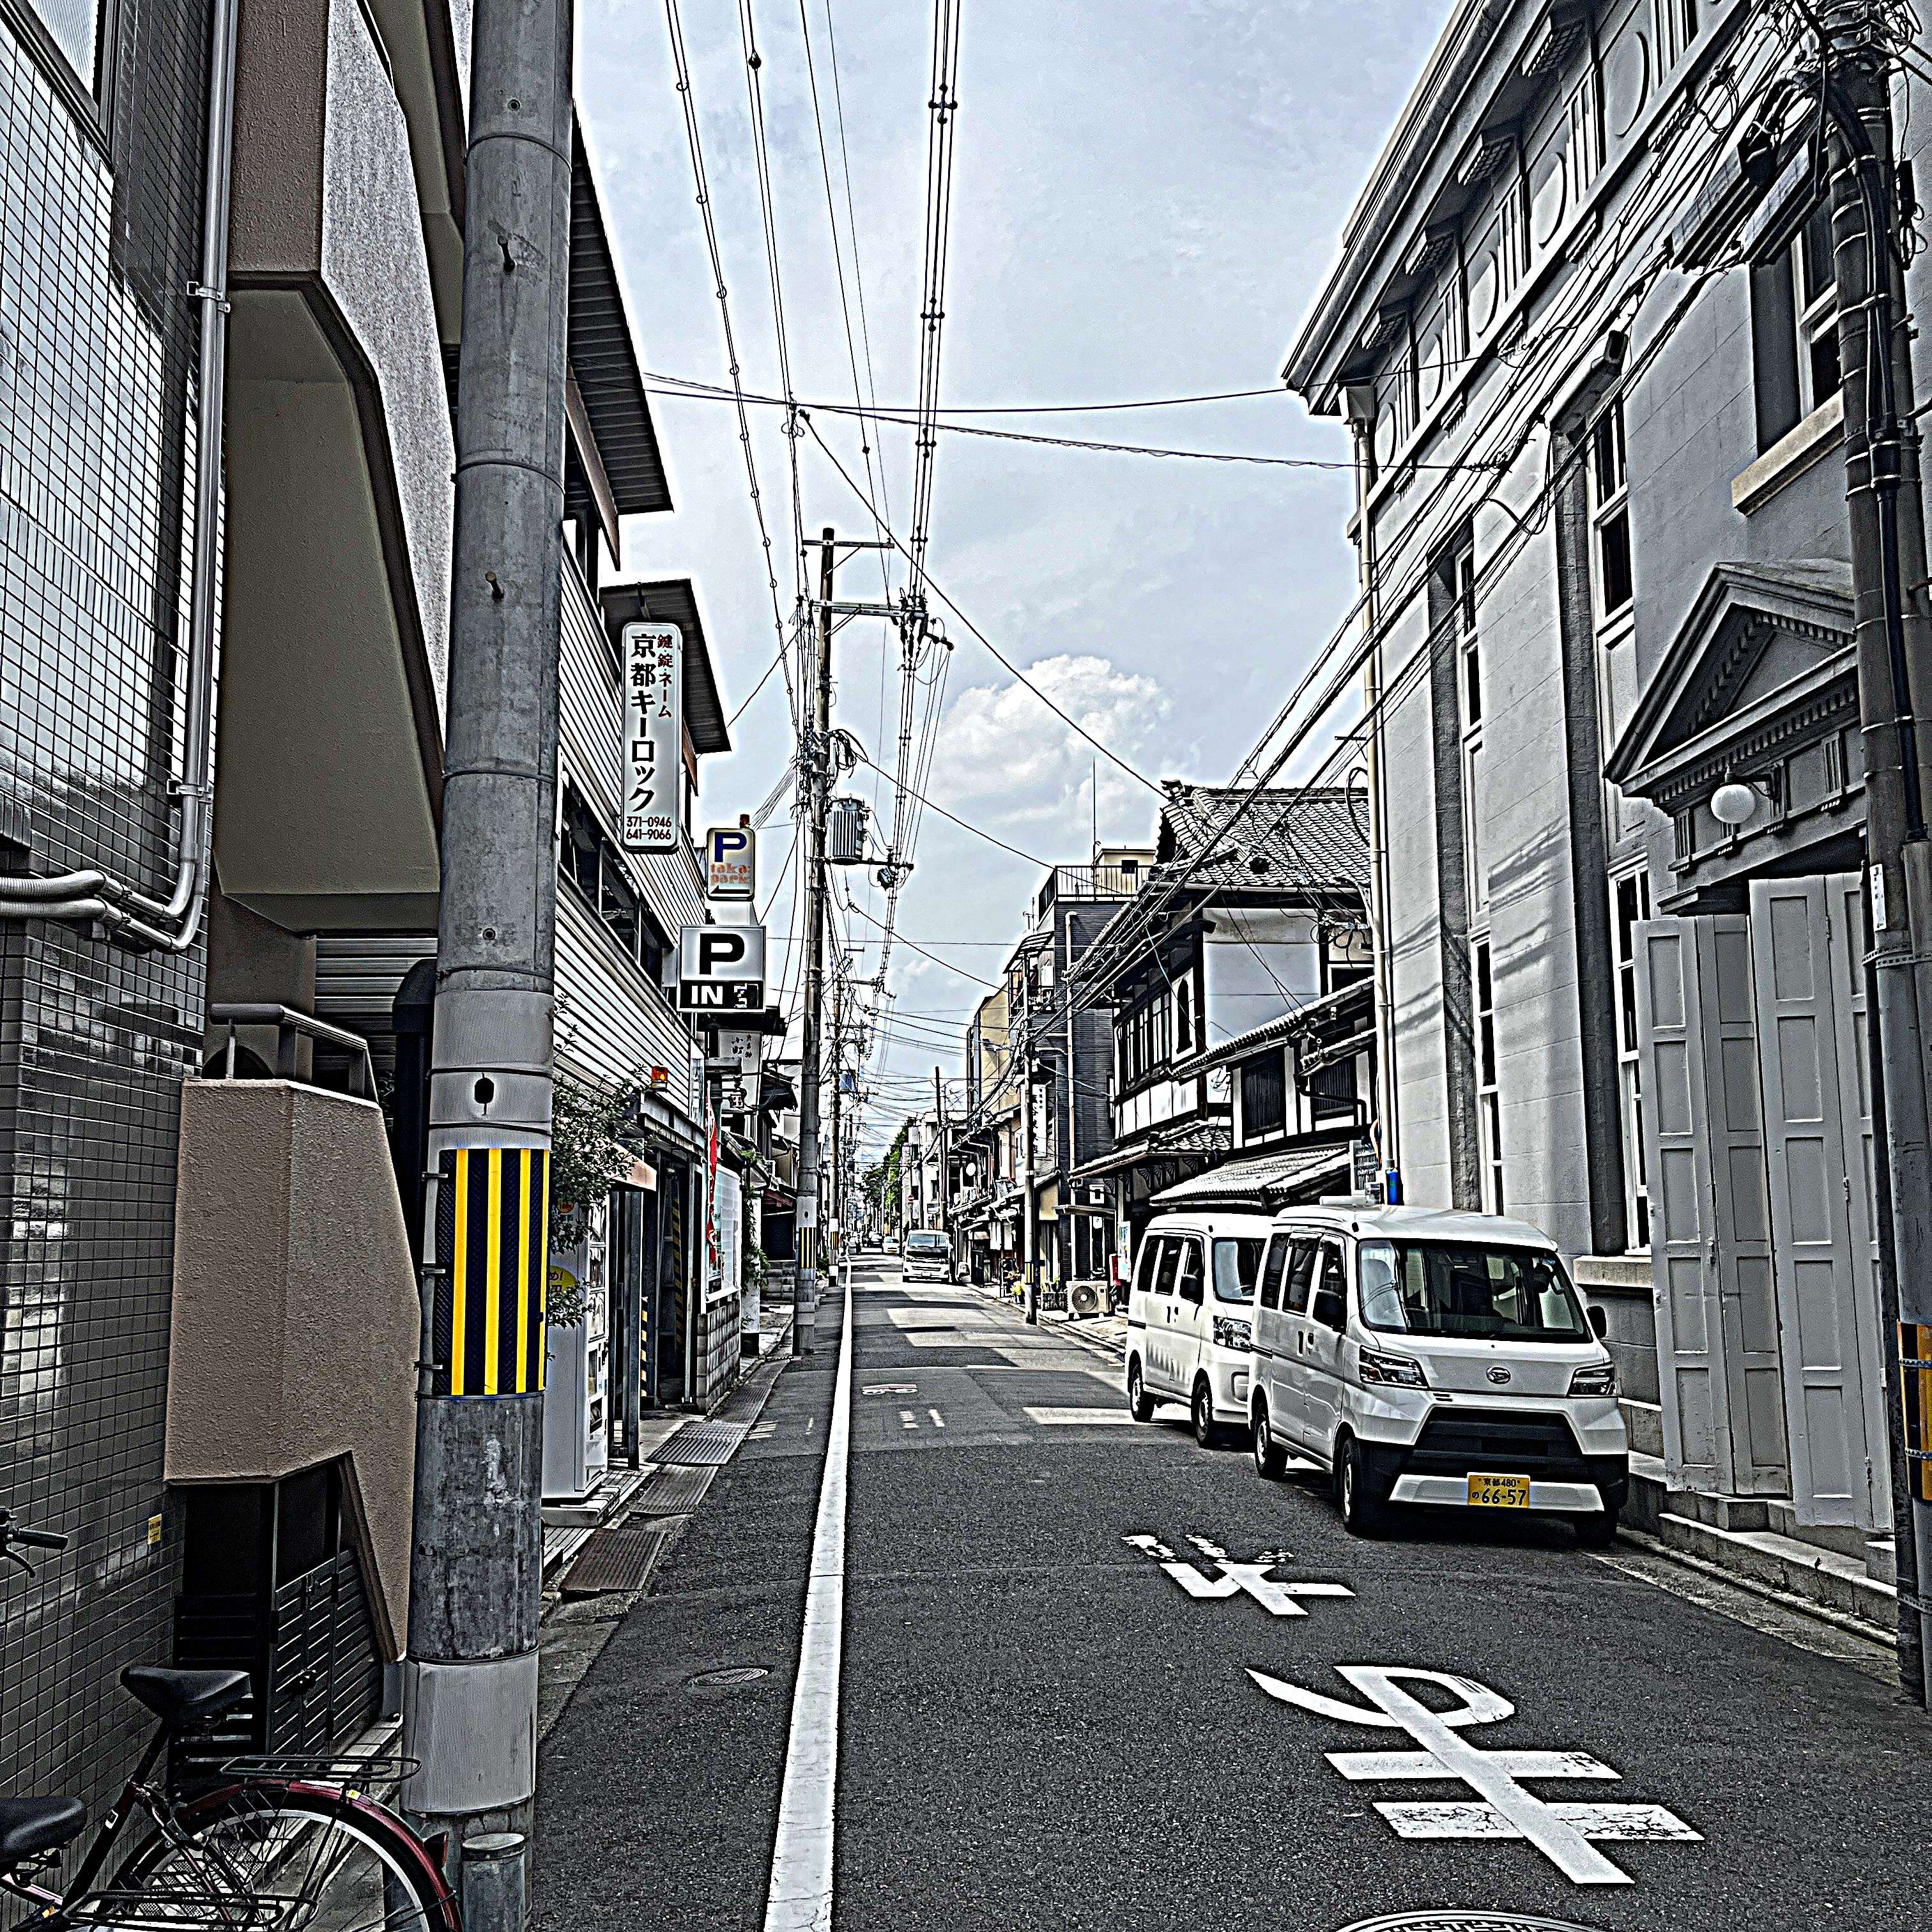
\includegraphics[width=0.2\linewidth]{../images/output/problem3/spatial/color4_3.0_50_8.3.png}}

    \caption{Unsharpening in Spatial Domain}

    \medskip

    \subfloat[color1]{\includegraphics[width=0.2\linewidth]{../images/output/problem3/frequency/color1_3.0_50_8.3.png}}
    \hspace{1pt}
    \subfloat[color3]{\includegraphics[width=0.2\linewidth]{../images/output/problem3/frequency/color3_3.0_50_8.3.png}}
    \hspace{1pt}
    \subfloat[color4]{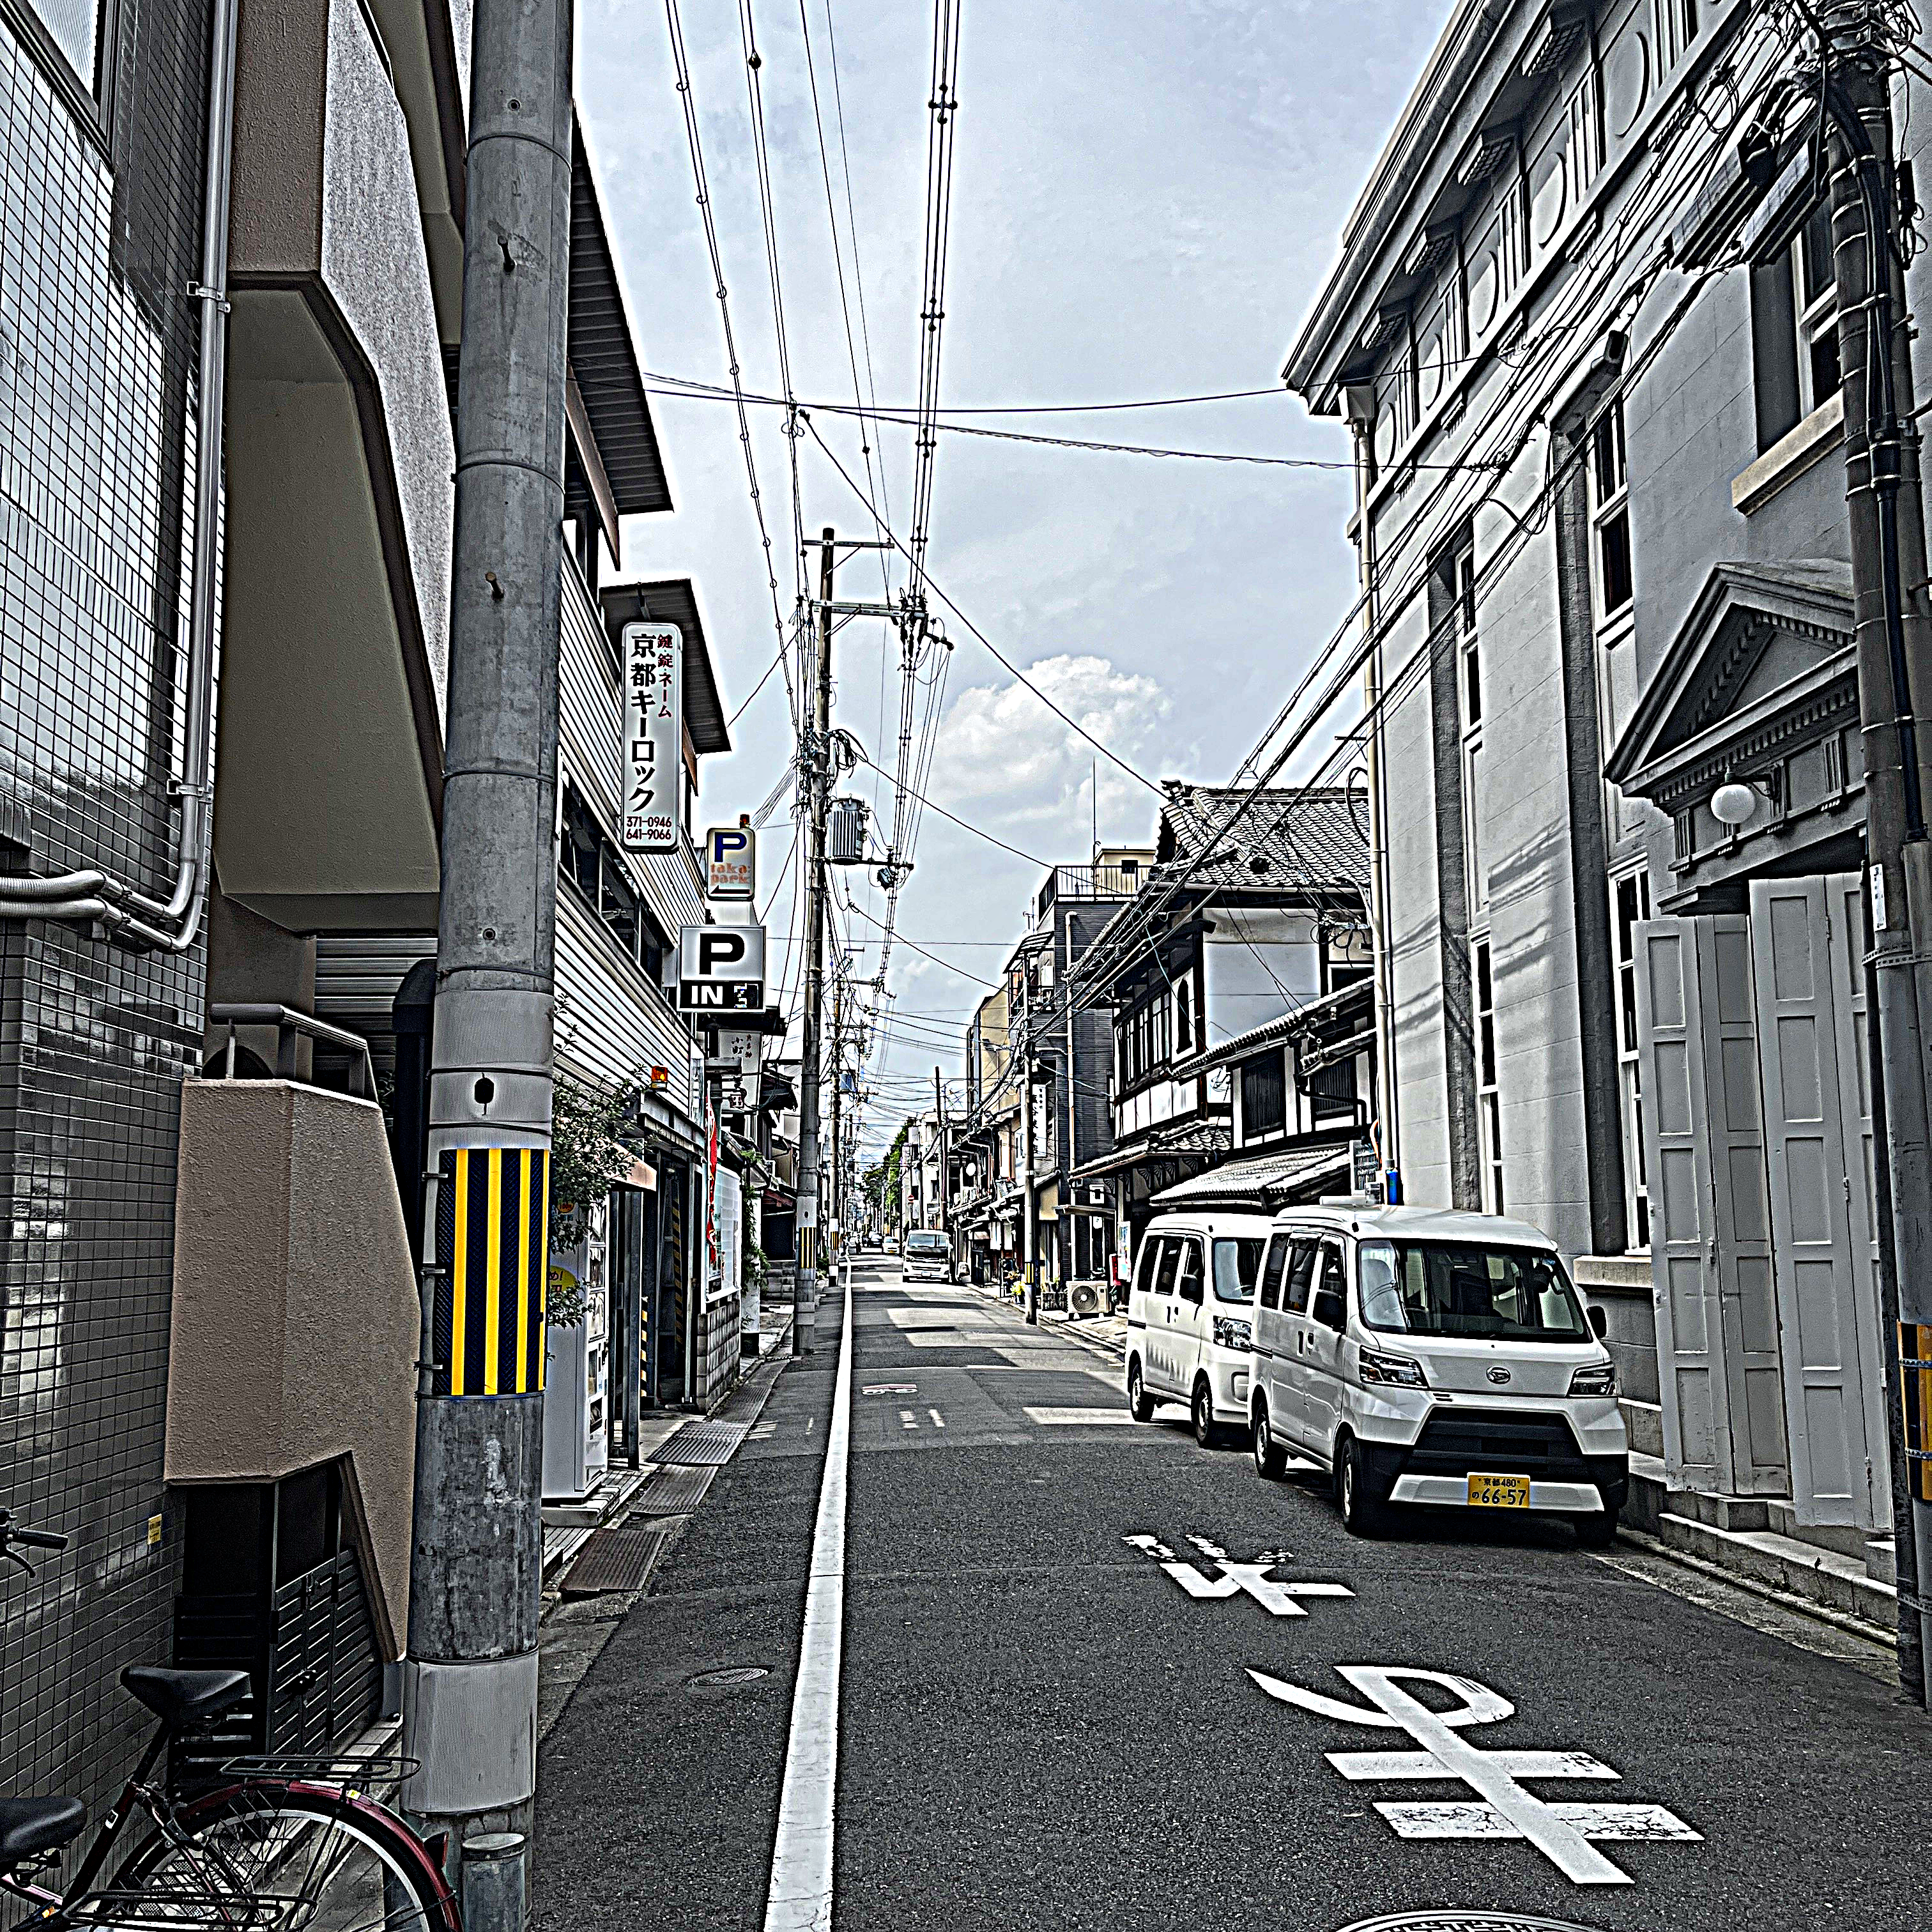
\includegraphics[width=0.2\linewidth]{../images/output/problem3/frequency/color4_3.0_50_8.3.png}}

    \caption{Unsharpening in Frequency Domain}
\end{figure}

\subsection*{Discussion}

\textbf{Effects of the parameters}

아래는 \code{alpha} 값에 따른 결과를 나타낸 것이다.
\code{alpha} 값이 증가함에 따라 경계값이 더욱 뚜렷해보임을 확인할 수 있다.

\begin{figure}[htbp]
    \centering

    \subfloat[alpha=1.0]{\includegraphics[width=0.25\linewidth]{../images/output/problem3/frequency/color3_1.0_50_8.3.png}}
    \hspace{1pt}
    \subfloat[alpha=2.0]{\includegraphics[width=0.25\linewidth]{../images/output/problem3/frequency/color3_2.0_50_8.3.png}}
    \hspace{1pt}
    \subfloat[alpha=3.0]{\includegraphics[width=0.25\linewidth]{../images/output/problem3/frequency/color3_3.0_50_8.3.png}}

    \caption{Effect of Alpha(padding=50,sigma=8.3,domain=frequency)}
\end{figure}

\newpage

Guassian Lowpass Filter의 Sigma는 수업자료에 따라 \code{padding/6.0}의 크기로 설정하여 필터링을 진행하였다.

아래는 \code{padding} 값에 따른 결과를 나타낸 것이다.
위에서 언급한대로, \code{sigma}는 \code{padding}에 의존하도록 설정되었다.
\code{sigma}의 값이 증가함에 따라 더욱 뚜렷한 결과를 보이는 것을 확인할 수 있다.

\begin{figure}[htbp]
    \centering

    \subfloat[padding=10]{\includegraphics[width=0.25\linewidth]{../images/output/problem3/frequency/color3_3.0_10_1.7.png}}
    \hspace{1pt}
    \subfloat[padding=25]{\includegraphics[width=0.25\linewidth]{../images/output/problem3/frequency/color3_3.0_25_4.2.png}}
    \hspace{1pt}
    \subfloat[padding=50]{\includegraphics[width=0.25\linewidth]{../images/output/problem3/frequency/color3_3.0_50_8.3.png}}

    \caption{Effect of Sigma(Padding)(alpha=3.0,domain=frequency)}
\end{figure}

아래는 \code{domain} 값에 따른 결과를 나타낸 것이다.
큰 차이를 확인할 수 없으며, Convolution Theorem을 확인할 수 있다.

\begin{figure}[htbp]
    \centering

    \subfloat[spatial]{\includegraphics[width=0.3\linewidth]{../images/output/problem3/spatial/color3_3.0_50_8.3.png}}
    \hspace{1pt}
    \subfloat[frequency]{\includegraphics[width=0.3\linewidth]{../images/output/problem3/frequency/color3_3.0_50_8.3.png}}

    \caption{Effect of Domain(padding=50,alpha=3.0,sigma=8.3)}
\end{figure}

\noindent{\textbf{Result of Each Step - Spatial Domain}}

다음은 Spatial Domain에서 Unsharpening에 따른 각 단계를 나타낸 그림이다.

\begin{figure}[htbp]
    \centering
    \subfloat[spatial]{\includegraphics[width=0.6\linewidth]{../images/output/problem3/spatial/analysis_color3_3.0_50_8.3.png}}
    \caption{Each Steps of Unsharpening - Spatial Domain}
\end{figure}

패딩된 이미지에 필터를 이용하여 Spatial Domain에서 Lowpass Filtering 진행 이후 해당 이미지를 기존 이미지에서 빼서 마지막 이미지의 High Frequency 이미지를 만든다.
High Frequency 이미지를 더해 Unsharpening을 진행한다.

\newpage

\noindent{\textbf{Result of Each Step - Frequency Domain}}

다음은 Frequency Domain에서 Unsharpening에 따른 각 단계를 나타낸 그림이다.

\begin{figure}[htbp]
    \centering
    \subfloat[Frequency]{\includegraphics[width=0.6\linewidth]{../images/output/problem3/frequency/analysis_color3_3.0_50_8.3.png}}
    \caption{Each Steps of Unsharpening - Frequency Domain}
\end{figure}

패딩된 이미지에서 각 채널별로 Frequency Domain으로 변환 후, Frequency Domain으로 변환된 Gaussian Filter를 적용해 Low Frequency를 필터링한다.
기존의 각 채널에서 Low Frequency 채널 이미지를 빼 High Frequency 채널을 얻은 이후, 이를 각 채널에 더해 Unsharpening을 한다.
마지막으로 Spatial Domain으로 변환하여 마무리한다.

\noindent{\textbf{Comparison Between the Spatial-Domain and Frequency-Domain}}

두 domain의 연산 시간 차이는 \code{padding} 크기 차이에 의해 발생한다.
각 domain의 시간복잡도를 계산하면 다음과 같다.

\begin{itemize}
    \item Spatial Domain: 각 픽셀별로 필터의 픽셀 수만큼 곱셈 연산이 필요하다.
    이후 Unsharpening에 따른 연산은 전체 이미지의 픽셀 수에 비례하는 계산 횟수를 가진다.
    이에 따라 전체 시간 복잡도는 $O(MN)$이 된다.
    이때, $M$과 $N$은 각각 필터의 픽셀 수, 이미지의 픽셀 수가 된다.

    \item Frequency Domain: Frequency Domain으로의 변환과 역변환에 대해 \code{numpy}에 의하면 $O(NlogN)$이 소요된다.
    Domain 변환 이후에는 연산마다 전체 이미지의 픽셀 수만큼 연산이 소요된다.
    따라서 전체 과정을 정리하면 $O(NlogN + N) = O(NlogN)$의 시간복잡도가 계산된다.
\end{itemize}

다음은 Domain에 따른 실제 연산에 걸린 시간을 정리한 표이다. (Color4.jpg, \code{alpha=3.0}, \code{padding=50}, \code{sigma=8.3})
Spatial Domain에서의 Unsharpening이 더 오래걸리는 것을 확인할 수 있다.

\begin{table*}[h]
    \centering
    \begin{tabular}{@{}cc@{}}
        \hline
        Domain & $T$ \\
        \hline
        Spatial & 270.14 \\
        Frequency & 3.50 \\
        \hline
    \end{tabular}
    \caption{Computational Time Depending on Domain}
\end{table*}

다음은 \code{padding}에 따른 연산 시간을 정리한 표이다. (Color4.jpg, \code{alpha=3.0})
Spatial Domain의 경우 \code{padding} 크기가 증가함에 따라 이미지에 대해 처리해야할 픽셀의 수가 늘어나 연산 시간 또한 늘어나는 것을 확인할 수 있다.
Frequency Domain 또한 증가하기는 하지만, Spatial Domain 대비 그 폭이 적은 것을 확인할 수 있다.

\begin{table*}[h]
    \centering
    \begin{tabular}{@{}cccc@{}}
        \hline
        Domain & $T_{10}$ & $T_{25}$ & $T_{50}$ \\
        \hline
        Spatial & 78.49 & 118.48 & 270.14 \\
        Frequency & 3.44 & 3.49 & 4.63 \\
        \hline
    \end{tabular}
    \caption{Computational Time Depending on Padding}
\end{table*}

\code{alpha} 값의 경우 연산 시간에 영향을 미치지 않는다.

\end{document}
